\documentclass[12pt,a4paper]{article}
\usepackage{amsmath}
\usepackage{amsfonts}
\usepackage{amssymb}
\usepackage{makeidx}
\usepackage{graphicx}
\usepackage{wrapfig}
\usepackage{enumerate}
\usepackage{pdfpages}
\usepackage{tocloft}
\usepackage{setspace}
\usepackage{mathtools}
\usepackage{hyperref}
\definecolor{linkcolour}{rgb}{0,0.2,0.6} % Link color
\hypersetup{colorlinks,breaklinks,urlcolor=linkcolour,linkcolor=linkcolour}
\usepackage[left=2cm,right=2cm,top=2cm,bottom=2cm]{geometry}

\usepackage{xcolor}
\usepackage{fontspec}
\setmainfont{Cambria}

\usepackage{subcaption}
\usepackage{caption}
\captionsetup[figure]{font=small, labelfont={bf}}
\captionsetup[table]{font=small, labelfont={bf}}

\usepackage{float}
\usepackage{multirow}
\usepackage{longtable}
\usepackage[nottoc]{tocbibind}

\usepackage{soul}

\newcommand{\spa}{\vspace{1.25em}}
\newcommand{\noi}{\noindent}
\def\dul#1{\underline{\underline{#1}}}
\def\cpt#1#2{{\begin{center}\small\textbf{\textcolor{blue}{Figure #1:}} #2\end{center}}}
\def\tt#1{\texttt{#1}}
% for dots in the content
\usepackage{tocloft}
\renewcommand{\cftsecleader}{\cftdotfill{\cftdotsep}}


\begin{document}
    \begin{titlepage} 
        \begin{center}
        \large{ASSIGNMENT 1}\\
        \vspace{2em}
        \large {CS5691 Pattern Recognition and Machine Learning}
        \vspace{3em}
        
        \rule{0.9\linewidth}{0.5mm} \\[0.4cm]
        {\Large{\bfseries{CS5691 Assignemnt 1}}} \\
        \rule{0.9\linewidth}{0.5mm} \\[3 em]    
        
        Team Members: \\
        \vspace{0.5em}
        \def\arraystretch{1.25}
\begin{tabular}{c l}
	\hline
	BE17B007 & N Sowmya Manojna \\
	PH17B010 & Thakkar Riya Anandbhai \\
	PH17B011 & Chaithanya Krishna Moorthy \\
	\hline
\end{tabular}

        \vspace{1em}

        Indian Institute of Technology, Madras\\    
        
        \vspace{5em}    
        
            
\includegraphics[scale = 0.09]{images/iitmlogo.png}
        \end{center}
    \end{titlepage}
{\hypersetup{linkcolor=black}
\tableofcontents}
\break

\section{Task 1}
\subsection{Mathematical Formulation}
The data for univariate polynomial regression is obtained by raising it to the required degree. In case of univariate polynomial regression of degree $d$, the dependent variable, of size $(d,1)$ is assumed to have the form
\begin{equation}
    \vec{y}_{n\times1} = \mathit{\phi}_{n\times d}W_{d\times1}
\end{equation}
\noi
The weights corresponding to a given degree is then calculated by using the closed form solution for univariate polynomial regression:
\begin{equation}
    W = (\mathit{\phi}^T\mathit{\phi} + \lambda \mathit{I})^{-1}\mathit{\phi}^T\vec{y}
\end{equation}
Where, $\lambda\mathit{I}$ is the regularization term.

\subsection{Training and Validation Accuracies}
In order to pick the parameters that best fit the dataset, a grid search was performed on the dataset. Prior to this, the dataset was split into training set, validation set and the testing set, in the ratio 70:10 (from the training data) :30. The results obtained is as follows:
\def\arraystretch{1.25}
\begin{center}
{\small
\begin{longtable}{l l l l l}
\hline
\hline
\textbf{$d$} & \textbf{$\lambda$} & \textbf{Train Error} & \textbf{Validation Error} \\
\hline
\hline
6 & 0.0 & 0.044889 & 0.159636 \\
3 & 0.0 & 0.672882 & 1.001484 \\
9 & 0.5 & 0.750020 & 1.469413 \\
2 & 0.0 & 1.014199 & 1.883134 \\
9 & 1.0 & 1.040132 & 1.929033 \\
9 & 2.0 & 1.354363 & 2.165779 \\
9 & 10.0 & 2.281929 & 1.857270 \\
9 & 50.0 & 3.342110 & 1.447933 \\
9 & 100.0 & 3.782560 & 1.380623 \\
9 & 0.0 & 5.063475 & 92.085167 \\
\hline
\caption{Results obtained for Task 1, with sample size of 10}
\end{longtable}
}
\end{center}

\vspace{-2em}\noi
Regularization was only applied in case of degree 9.\\

\def\arraystretch{1.25}
\begin{longtable}{l l l l l}
\hline
\hline
\textbf{Degree} & \textbf{$\lambda$} & \textbf{Train Error} & \textbf{Validation Error} \\
\hline
\hline
6 & 0.0 & 0.094536 & 0.094379 \\
9 & 0.0 & 0.093581 & 0.100752 \\
9 & 0.5 & 0.134226 & 0.152565 \\
9 & 1.0 & 0.186479 & 0.209008 \\
9 & 2.0 & 0.289107 & 0.311716 \\
9 & 10.0 & 0.766298 & 0.776521 \\
3 & 0.0 & 0.934079 & 0.862605 \\
2 & 0.0 & 1.591842 & 1.421021 \\
9 & 50.0 & 1.620063 & 1.707757 \\
9 & 100.0 & 2.138200 & 2.310223 \\
\hline
\caption{Results obtained for Task 1, with sample size of 200}
\end{longtable}
\noi
\textcolor{blue}{From the table above, we see that the best fit for the data is obtained for degree: $6$ and $\lambda:0$.}

\subsection{Model Fits}
\subsubsection{Sample Size: 10}
The polynomial models and the corresponding fits obtained for sample size of 10 are as follows:
\begin{figure}[H]
    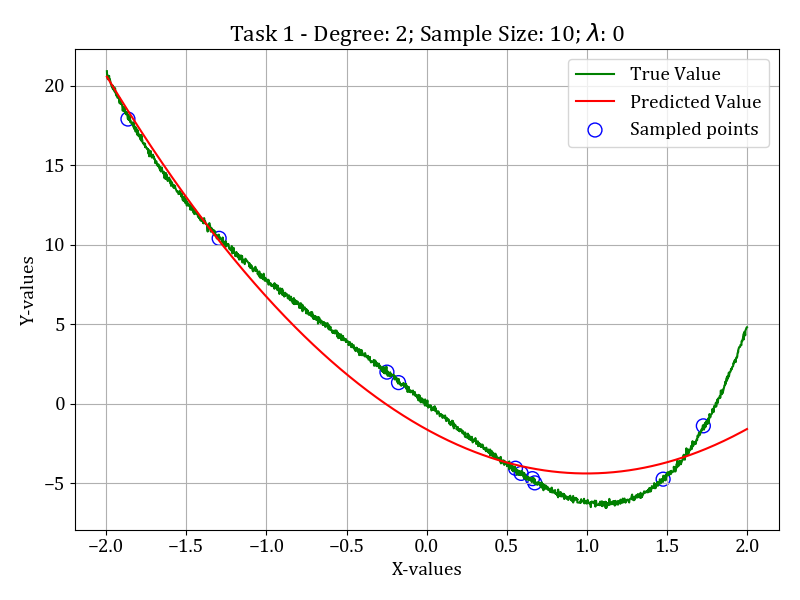
\includegraphics[scale=0.425]{images/t1_d1/d_2_size_10_l_0.png}
    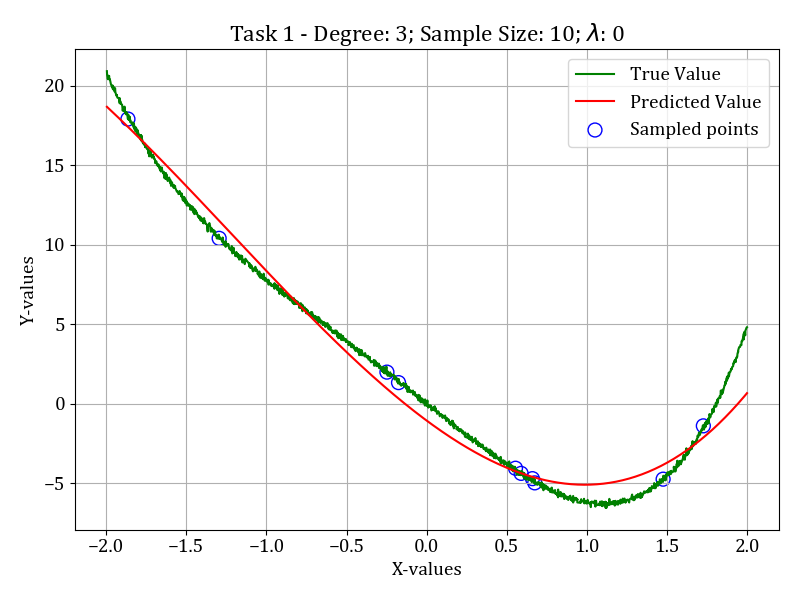
\includegraphics[scale=0.425]{images/t1_d1/d_3_size_10_l_0.png}
    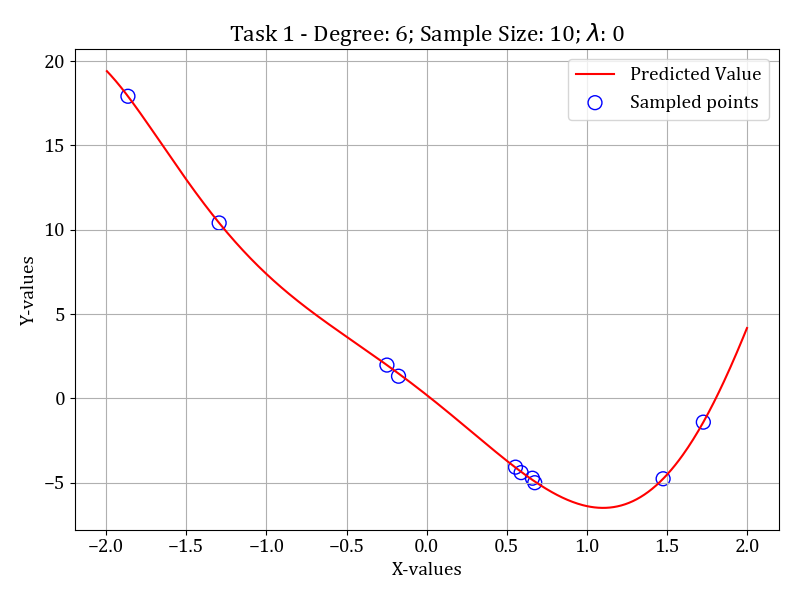
\includegraphics[scale=0.425]{images/t1_d1/d_6_size_10_l_0.png}
    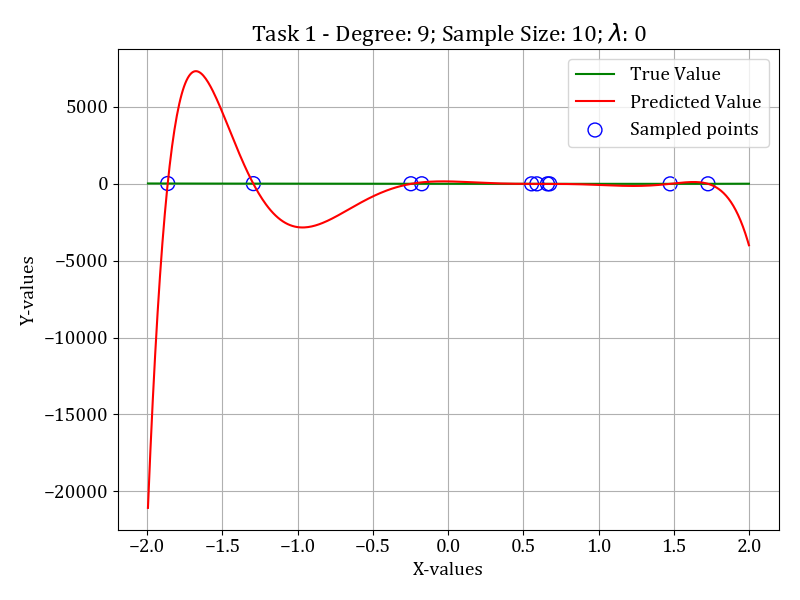
\includegraphics[scale=0.425]{images/t1_d1/d_9_size_10_l_0.png}
    \caption{Task 1 - Polynomial fits, Sample size: 10}
\end{figure}

\subsubsection{Sample Size: 200}
The polynomial models and the corresponding fits obtained for sample size of 200 are as follows:
\begin{figure}[H]
    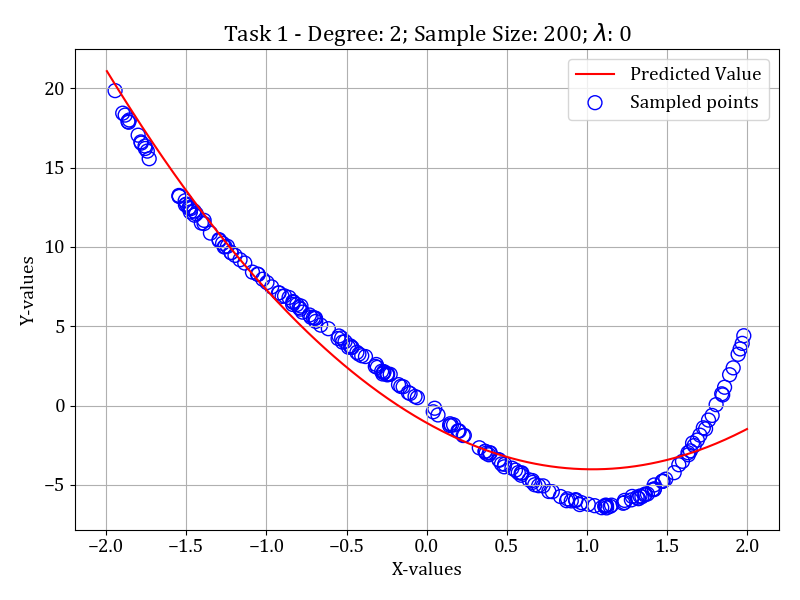
\includegraphics[scale=0.425]{images/t1_d1/d_2_size_200_l_0.png}
    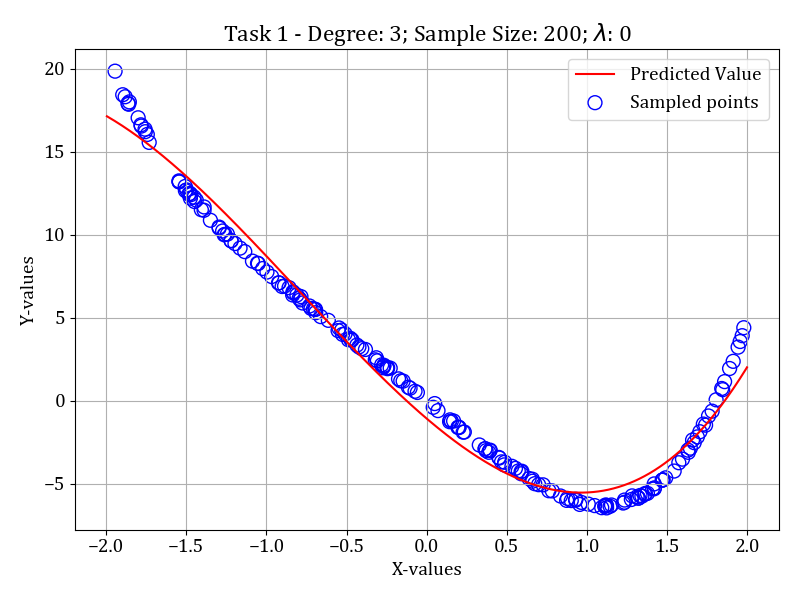
\includegraphics[scale=0.425]{images/t1_d1/d_3_size_200_l_0.png}
    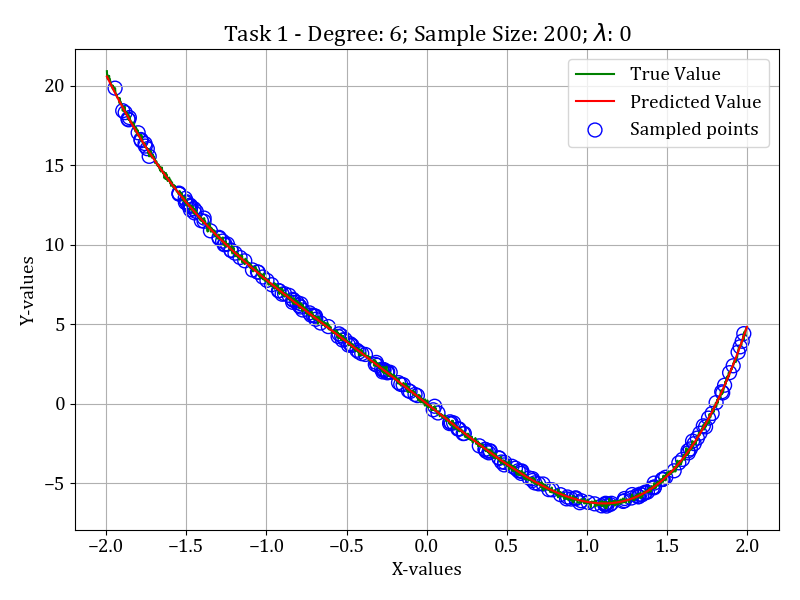
\includegraphics[scale=0.425]{images/t1_d1/d_6_size_200_l_0.png}
    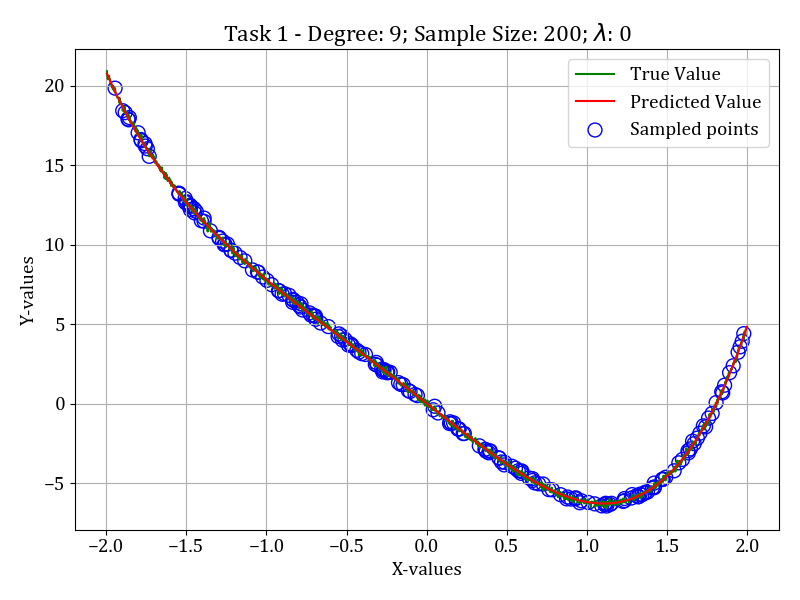
\includegraphics[scale=0.425]{images/t1_d1/d_9_size_200_l_0.png}
    \caption{Task 1 - Polynomial fits, Sample size: 200}
\end{figure}

\subsubsection{Effects of Regularization}
The polynomial models and the corresponding fits obtained for sample size of 10, across different $\lambda$ values are as follows:
\begin{figure}[H]
    \ContinuedFloat
    \begin{subfigure}{\textwidth}
    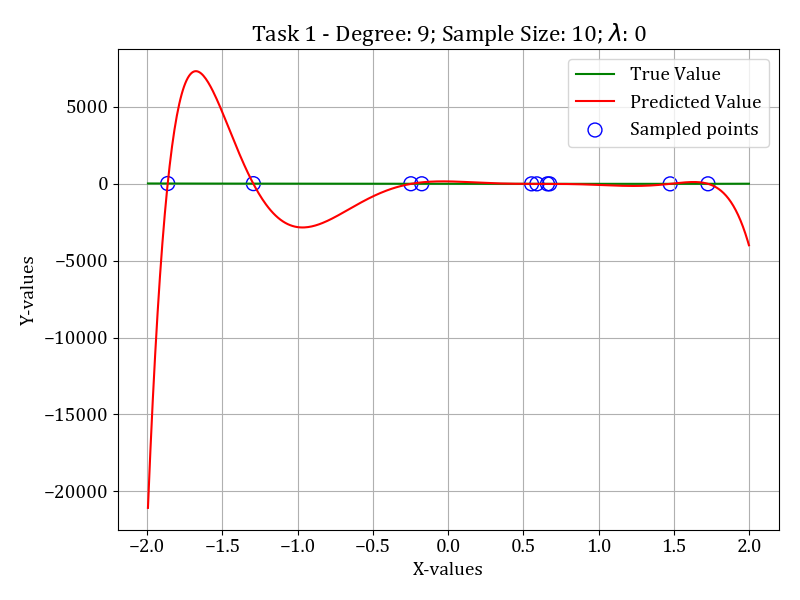
\includegraphics[scale=0.45]{images/t1_d1/d_9_size_10_l_0.png}
    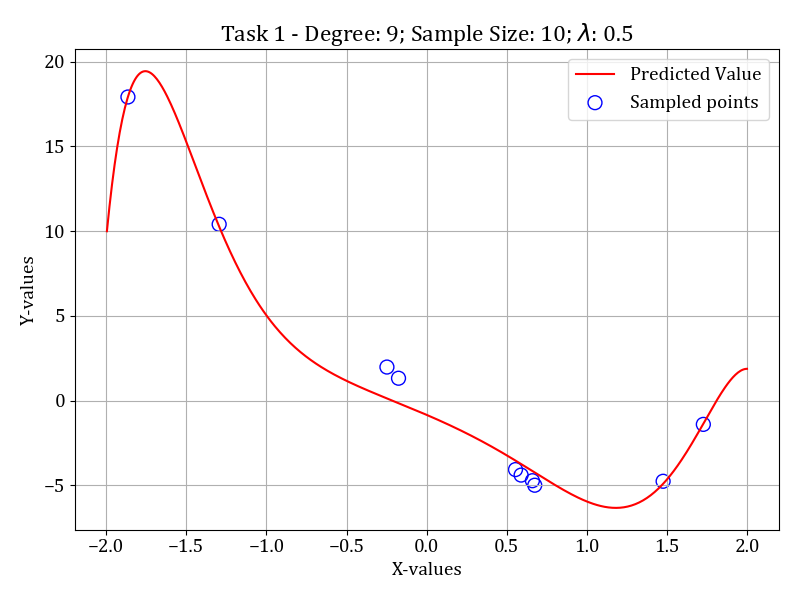
\includegraphics[scale=0.45]{images/t1_d1/d_9_size_10_l_0.5.png}
    \end{subfigure}
    \ContinuedFloat
    \begin{subfigure}{\textwidth}
    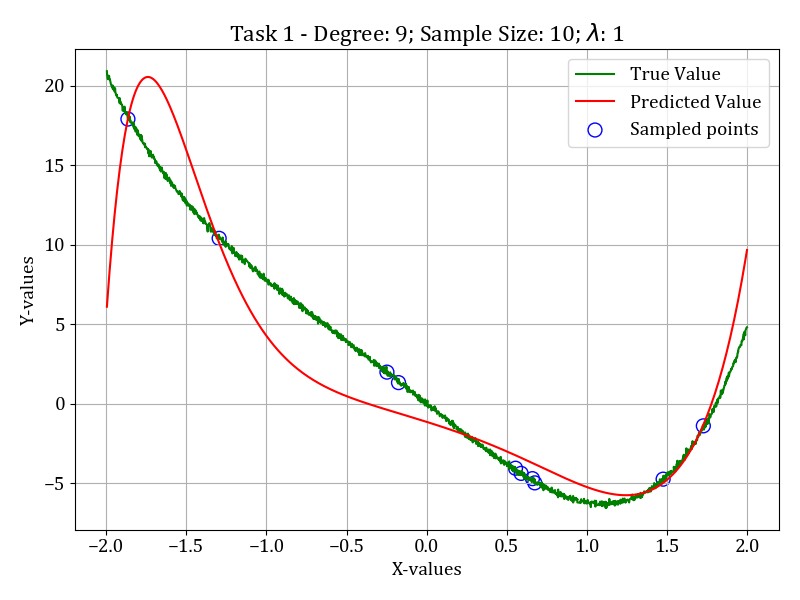
\includegraphics[scale=0.45]{images/t1_d1/d_9_size_10_l_1.png}
    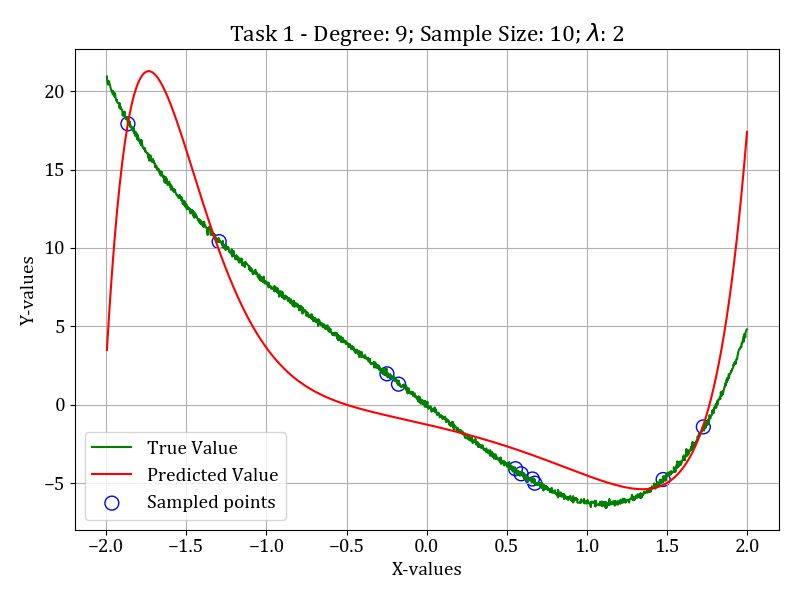
\includegraphics[scale=0.45]{images/t1_d1/d_9_size_10_l_2.png}
    \end{subfigure}
    \ContinuedFloat
    \begin{subfigure}{\textwidth}
    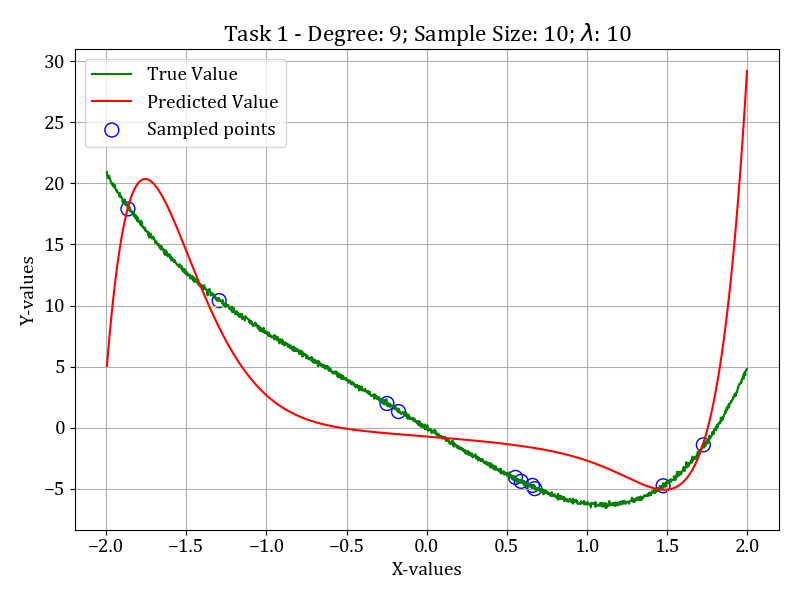
\includegraphics[scale=0.45]{images/t1_d1/d_9_size_10_l_10.png}
    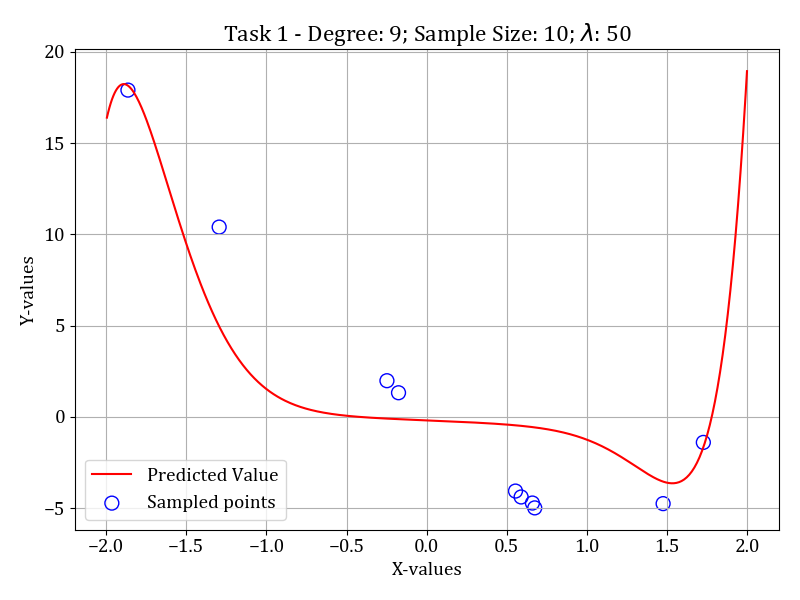
\includegraphics[scale=0.45]{images/t1_d1/d_9_size_10_l_50.png}
    \end{subfigure}
    \ContinuedFloat
    \begin{subfigure}{\textwidth}
    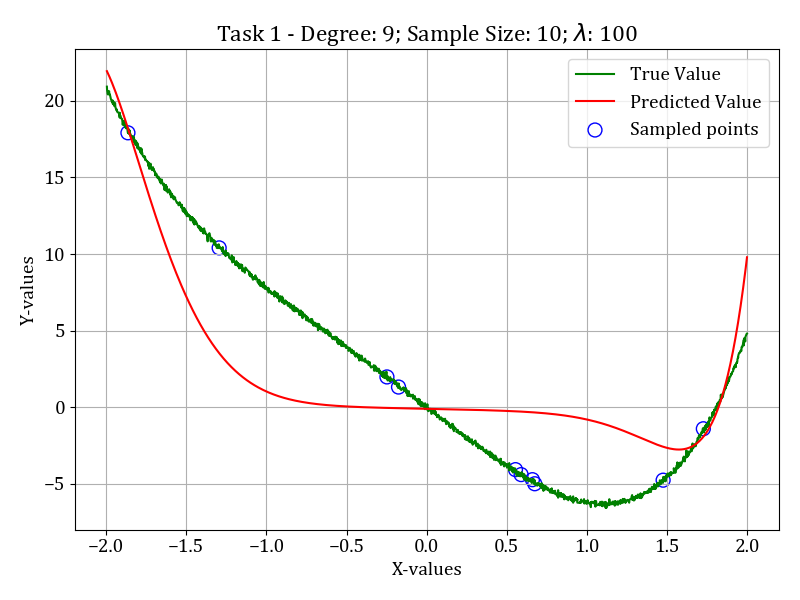
\includegraphics[scale=0.45]{images/t1_d1/d_9_size_10_l_100.png}
    \end{subfigure}
    \caption{Task 1 - 9\textsuperscript{th} Degree Polynomial fit, Sample size: 10}
\end{figure}

\subsection{Best Model}
The best fit, $d:6$ and $\lambda:0$ is visualized as follows:
\begin{figure}[H]
    \centering
    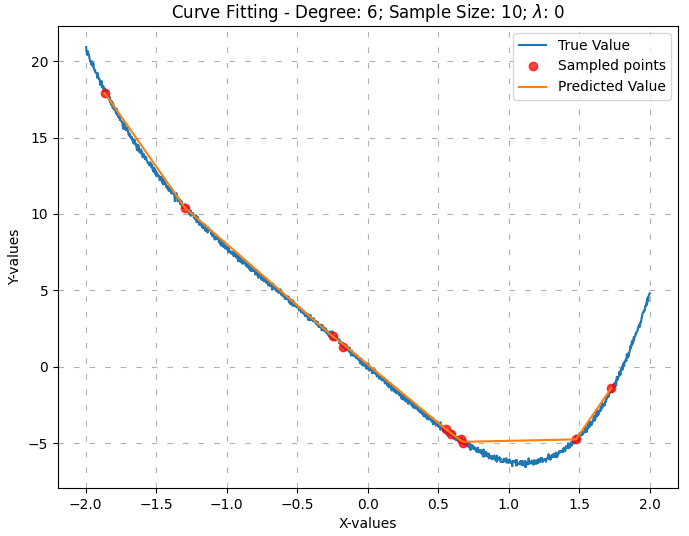
\includegraphics[scale=0.5]{images/d_6_size_10_l_0.png}
    \caption{Task 1 - Best fit, Sample size: 10}
\end{figure}
\begin{figure}[H]
    \centering
    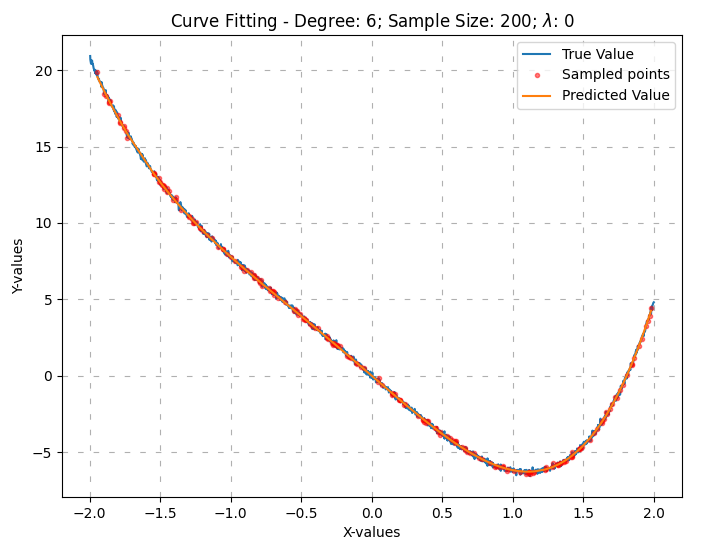
\includegraphics[scale=0.5]{images/d_6_size_200_l_0.png}
    \caption{Task 1 - Best fit, Sample size: 200}
\end{figure}
\noi
The final training and testing error obtained is as follows:
\begin{itemize}
    \itemsep0em
    \item Training Error: 0.09974659089780814
    \item Testing Error: 0.09793071099285168
\end{itemize}

\section{Task 2}
\subsection{Polynomial Regression for bivariate data}
The second dataset is a bivariate data with 2000 examples. We assume that the target variable is of the form:
\begin{equation}
\label{eq:1}
    y=\sum_{i=0}\omega _{i}\phi_{i}(x_1,x_2)  +\epsilon 
\end{equation}
Where $\omega_{i}$ are the parameters to be found through regression, $\phi_{i}(x_1,x_2)$ is a polynomial in $x_1$ and $x_2$ and $\epsilon$ is the normally distributed error.\\ 

\noi
A breakdown of the steps undertaken is:
\begin{itemize}
    \itemsep0em
    \item The function \tt{create\_phi} generates the design matrix $\phi(x_1,x_2)$ for the required degree of complexity.
    \item The design matrix is passed to the function \tt{regularized\_pseudo\_inv}, which generates the Moore-Penrose inverse of the given design matrix (X) and specified value of regularization parameter lambda ($\lambda$).
    
    \begin{equation}
         (X^T X + \lambda I)^{-1}X^T
    \end{equation}
    
    \item The function \tt{opt\_regularized\_param} is then used to obtain optimum values of $\vec{\omega}$
    \begin{equation}
        \vec{\omega} = [(X^T X + \lambda I)^{-1}X^T]y
    \end{equation}
    Where $y$ is the output as defined in the \autoref{eq:1}.
    
    \item The optimum parameter vector thus obtained can be used to predict the variable $y$ for new inputs. 
    \begin{equation}
        y_{prediction}=X\vec{\omega}
    \end{equation}
\end{itemize}

\subsection{Data processing}
\begin{itemize}
    \itemsep0em
    \item The range of variables is same for $x_1$ and $x_2$, (i.e.) $(-16,16)$ hence no scaling is required, there are no null data values.
    \item The data is first shuffled and then split into Train data, Cross-validation data and Test data. Train data sizes: $50, 200, 500$
    \item The independent vectors $\vec{x_1}$ and $\vec{x_2}$ are extracted from the datasets and then design matrices $\phi_{n\times m}$ are created using the function \tt{create\_phi}. Here, $n$ is the number of samples in the respective sample and $m$ is the number of components for the corresponding degree.
\end{itemize}

\subsection{Degree of complexity 2}
With degree of complexity set to 2, for a particular data point, 
\begin{equation}
y_{i}=\omega_{0}+\omega_{1}x_1 + \omega_{2}x_2 + \omega_{3}{x_1}^2+\omega_{4}{x_2}^2+\omega_{5}{x_1}{x_2}
\end{equation}

 
\subsubsection{Varying $\lambda$, Sample size of 50}
After the above pre-processing, The optimum parameter \textbf{$\vec{\omega}$} is obtained for the following lambda values - $[0, 0.5, 1, 2, 10, 50, 100]$. The variation in RMSE across lambda is as follows:\\
 
\begin{figure}[H]
     \centering
     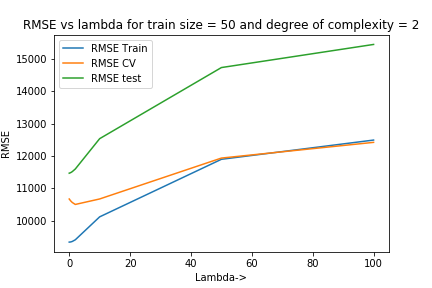
\includegraphics[scale=0.7]{images/d2_50.png}
     \caption{RMSE across $\lambda$; Sample size: 50,  Degree: 2}
\end{figure}
 
 
\begin{center}
\begin{tabular}{c c c c} 
\hline
\hline
\textbf{Lambda} & \textbf{RMSE Train} & \textbf{RMSE CV} & \textbf{RMSE Test} \\
\hline
\hline
0 & 9340.73 & 10671.59 & 11468.19 \\ 
0.5 & 9346.19 & 10611.41 & 11487.13 \\
1 & 9361.17 & 10564.66 & 11516.49 \\
\hl{2} & \hl{9412.58} & \hl{10503.67} & \hl{11598.33} \\
10 & 10120 & 10672.93 & 12534.16 \\
50 & 11897.56 & 11935.27 & 14729.56  \\ 
100 & 12491.10 & 12420.38 & 15443.04 \\ 
\hline
\end{tabular}
\captionof{table}{Variation in RMSE values with lambda}\label{d250}
\end{center}
\subsubsection{Varying $\lambda$, Sample size of 200}
 
 The optimum parameter \textbf{$\vec{\omega}$} is obtained for the following lambda values - $[0, 0.5, 1, 2, 10, 50, 100]$. The variation in RMSE across lambdas is as follows: \\
 
\begin{figure}[H]
     \centering
     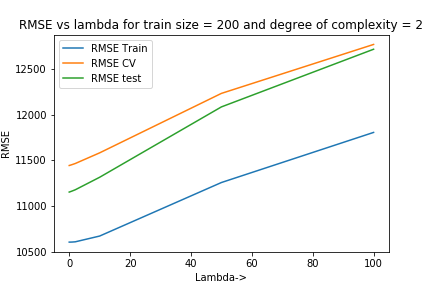
\includegraphics[scale=0.7]{images/d2_200.png}
     \caption{RMSE across $\lambda$; Sample size: 200, Degree: 2}
\end{figure}
 
 
\begin{center}
\begin{tabular}{c c c c} 
\hline
\hline
\textbf{Lambda} & \textbf{RMSE Train} & \textbf{RMSE CV} & \textbf{RMSE Test} \\
\hline
\hline
0 & 10 & 10671.59 & 11468.19 \\ 
0.5 & 9346.19 & 10611.41 & 11487.13 \\
1 & 9361.17 & 10564.66 & 11516.49 \\
\hl{2} & \hl{9412.58} & \hl{10503.67} & \hl{11598.33} \\
50 & 11897.56 & 11935.27 & 14729.56  \\ 
100 & 12491.10 & 12420.38 & 15443.04 \\
\hline
\end{tabular}
\captionof{table}{Variation in RMSE values with lambda}\label{d250}
\end{center}
 
\subsubsection{Varying $\lambda$, Sample size of 500}
\begin{figure}[H]
     \centering
     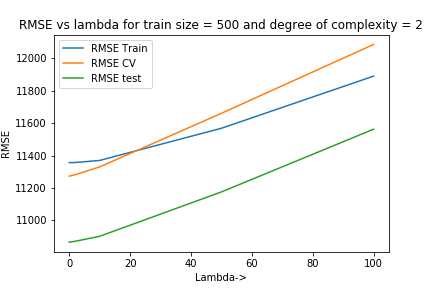
\includegraphics[scale=0.7]{images/d2_500.png}
     \caption{RMSE across $\lambda$; Sample size: 500, Degree: 2}
     \label{fig:d2500}
\end{figure}
 



\subsection{Degree of complexity 3}
With degree of complexity set to 3, for a particular data point, 
\begin{equation}
y_{i}=\omega_{0}+\omega_{1}{x_1}+\omega_{2}{x_2}+\omega_{3}{x_1}^2+\omega_{4}{x_2}^2+\omega_{5}{x_1}.{x_2}+\omega_{6}{x_1}^{3}+\omega_7{x_2}^{3}+\omega_8{x_2}^2{x_1}+\omega_9{x_1}^2{x_2}  
\end{equation}

\subsubsection{Varying $\lambda$, Sample size of 50}
 
After the above pre processing, The optimum parameter \textbf{$\vec{\omega}$} is obtained for the following lambda values - $[0, 0.5, 1, 2, 10, 50, 100]$. The variation in RMSE across lambdas is as follows:
\def\arraystretch{1.25}
\begin{center}
\begin{tabular}{l l l l}
\hline
\hline
\textbf{Lambda} & \textbf{RMSE Train} & \textbf{RMSE CV} & \textbf{RMSE Test} \\
\hline
\hline
0.0 & 8407.761210828727 & 11960.392166857815 & 12390.588660098681 \\
0.5 & 8414.299614637861 & 11743.19358761457 & 12329.126658336485 \\
1.0 & 8431.988457444206 & 11558.772331311482 & 12293.299535838765 \\
2.0 & 8491.472017549635 & 11270.79171291384 & 12280.362852665143 \\
\hl{10.0} & \hl{9240.199538933726} & \hl{10757.219031210356} & \hl{13112.100832682248} \\
50.0 & 10876.901176573218 & 12040.04490493105 & 15628.464519645266 \\
100.0 & 11379.791399813128 & 12642.949547533039 & 16474.271301190667 \\
\hline
\end{tabular}
\captionof{table}{Results obtained for Task 2}
\end{center}


\begin{figure}[H]
     \centering
     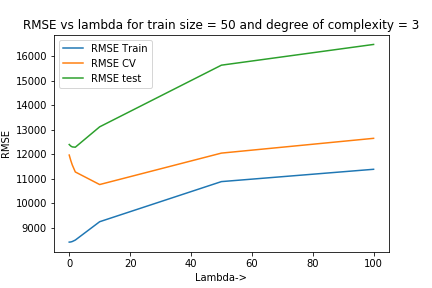
\includegraphics[scale=0.7]{images/d3_50.png}
     \caption{RMSE across $\lambda$; Sample size: 50, Degree: 3}
     \label{fig:d350}
\end{figure}
 
\subsubsection{Varying $\lambda$, Sample size of 200}
The obtained results are:
\def\arraystretch{1.25}
\begin{center}
\begin{tabular}{l l l l}
\hline
\hline
\textbf{Lambda} & \textbf{RMSE Train} & \textbf{RMSE CV} & \textbf{RMSE Test} \\
\hline
\hline
0.0 & 10322.506441224592 & 11480.65137585371 & 11540.748956514151 \\
0.5 & 10322.74337910385 & 11484.060426748905 & 11548.276365031981 \\
1.0 & 10323.437876912261 & 11487.78843512935 & 11556.1380959018 \\
2.0 & 10326.106384432025 & 11496.129590042878 & 11572.780261162094 \\
10.0 & 10392.059429467075 & 11592.560024074122 & 11735.150238100397 \\
50.0 & 10984.962331062083 & 12191.950852364467 & 12578.93878751002 \\
100.0 & 11522.792243145757 & 12692.364674117875 & 13234.250404753897 \\
\hline
\end{tabular}
\captionof{table}{Results obtained for Task 2}
\end{center}

\noi
Scatter plots of the model prediction using the regularization parameter value 0.01:
 
\begin{figure}[H]
     \centering
     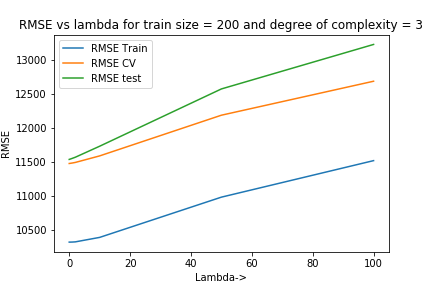
\includegraphics[scale=0.7]{images/d3_200.png}
     \caption{RMSE across $\lambda$; Sample size: 200, Degree: 3}
     \label{fig:d3200}
\end{figure}
 
\subsubsection{Varying $\lambda$, Sample size of 500}
 
The optimum parameter \textbf{$\vec{\omega}$} is obtained for the following lambda values - $[0, 0.5, 1, 2, 10, 50, 100]$.  The variation in RMSE across lambdas is as follows: \\
 
\begin{figure}[H]
     \centering
     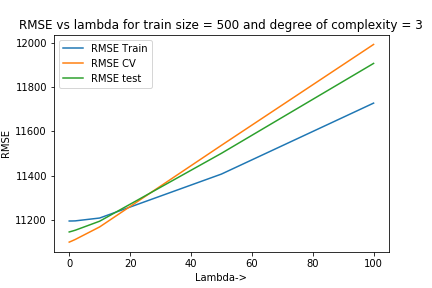
\includegraphics[scale=0.7]{images/d3_500.png}
     \caption{RMSE across $\lambda$; Sample size: 500, Degree: 3}
     \label{fig:d3500}
\end{figure}
 
\subsection{Degree of complexity 6}

With the degree of complexity 6, 
\begin{equation}
    y=\sum {x_1}^\alpha*{x_2}^\beta
\end{equation}
Where $0\leq\alpha+\beta\leq6$.
\subsubsection{Varying $\lambda$, Sample size of 50}
\def\arraystretch{1.25}
\begin{center}
\begin{tabular}{l l l l}
\hline
\hline
\textbf{Lambda} & \textbf{RMSE Train} & \textbf{RMSE CV} & \textbf{RMSE Test} \\
\hline
\hline
0.0 & 1.3582344908807028e-07 & 1.3024937374699014e-07 & 2.736466435265001e-07 \\
0.5 & 5.3224862846108924e-05 & 0.0006389419451237852 & 0.0011697424661700818 \\
1.0 & 0.00010241277566647342 & 0.001259472447857696 & 0.0022735033897776087 \\
2.0 & 0.00019571426483158983 & 0.002466786482370453 & 0.00436957859101229 \\
10.0 & 0.0009066540184949185 & 0.011454915983379615 & 0.0195422946271592 \\
50.0 & 0.004319989638299114 & 0.049682786993700954 & 0.08571221964007386 \\
100.0 & 0.008418172149435164 & 0.09086562659012756 & 0.15931182940985875 \\
\hline
\end{tabular}
\captionof{table}{Results obtained for Task 2}
\end{center}


\begin{figure}[H]
     \centering
     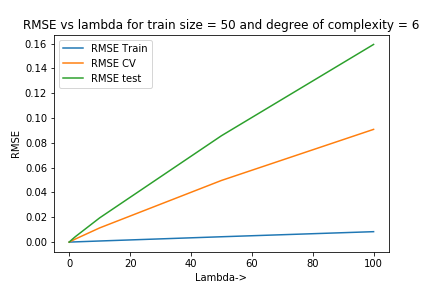
\includegraphics[scale=0.7]{images/d6_50.png}
     \caption{RMSE across $\lambda$; Sample size: 50, Degree: 6}
     \label{fig:d650}
\end{figure}
 

\subsubsection{Varying $\lambda$, Sample size of 200}
\def\arraystretch{1.25}
\begin{center}
\begin{tabular}{l l l l}
\hline
\hline
\textbf{Lambda} & \textbf{RMSE Train} & \textbf{RMSE CV} & \textbf{RMSE test} \\
\hline
\hline
0.0 & 4.145074549079158e-08 & 4.5876133577776055e-08 & 4.438277930933977e-08 \\
0.5 & 7.169634585154078e-06 & 9.351643870044926e-06 & 1.2226632701546666e-05 \\
1.0 & 1.4193629639985923e-05 & 1.852785190860779e-05 & 2.42010151174377e-05 \\
2.0 & 2.789871866381927e-05 & 3.649449750964621e-05 & 4.7603283521130243e-05 \\
10.0 & 0.000128403762827723 & 0.0001679510933427838 & 0.000216489022423017 \\
50.0 & 0.0005954210072570998 & 0.0007608482959799609 & 0.0009543646518816395 \\
100.0 & 0.0011768765498580448 & 0.0014847238097789764 & 0.001842159446862891 \\
\hline
\end{tabular}
\captionof{table}{Results obtained for Task 2}
\end{center}



\begin{figure}[H]
     \centering
     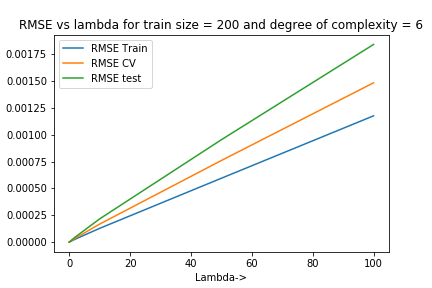
\includegraphics[scale=0.7]{images/d6_200.png}
     \caption{RMSE across $\lambda$; Sample size: 200, Degree: 6}
     \label{fig:d200}
\end{figure}
 
\subsubsection{Varying $\lambda$, Sample size of 500 }
\def\arraystretch{1.25}
\begin{center}
\begin{tabular}{l l l l}
\hline
\hline
\textbf{Lambda} & \textbf{RMSE Train} & \textbf{RMSE CV} & \textbf{RMSE test} \\
\hline
\hline
0.0 & 3.540887282123727e-08 & 3.741549292426492e-08 & 3.4517606283226707e-08 \\
0.5 & 2.4891560253931053e-06 & 2.69805964526573e-06 & 2.5949552832042936e-06 \\
1.0 & 4.963649710534798e-06 & 5.3778590424185165e-06 & 5.176457054060217e-06 \\
2.0 & 9.866381792471788e-06 & 1.069014286492481e-05 & 1.0291657829414182e-05 \\
10.0 & 4.744117748092903e-05 & 5.148944778527705e-05 & 4.9743962467771885e-05 \\
50.0 & 0.00021913097081968563 & 0.00023736669064951702 & 0.00023193961964998602 \\
100.0 & 0.00042714320882117563 & 0.00046046329475841634 & 0.0004529678734930164 \\
\hline
\end{tabular}
\captionof{table}{Results obtained for Task 2}
\end{center}


 
\begin{figure}[H]
     \centering
     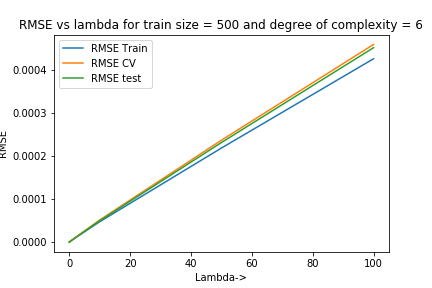
\includegraphics[scale=0.7]{images/d6_500.png}
     \caption{RMSE across $\lambda$; Sample size: 500, Degree: 6}
     \label{fig:d6500}
\end{figure}
 
\subsection{Conclusion}
 
 The RMSE values are least over train data, cross-validation data as well as test data for degree of complexity = 6, train data size = 500 and regularization parameter, lambda =0.
 
\begin{figure}[H]
     \centering
     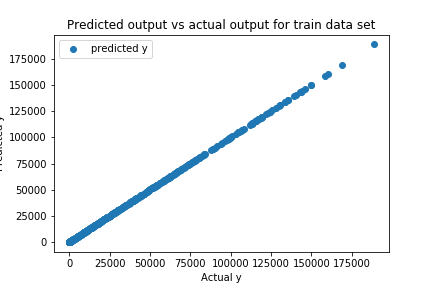
\includegraphics[scale=0.7]{images/predgoodtrain.png}
     \caption{Predicted output, Actual values for Train Data}
     \label{fig:d6500}
\end{figure}
 
\begin{figure}[H]
     \centering
     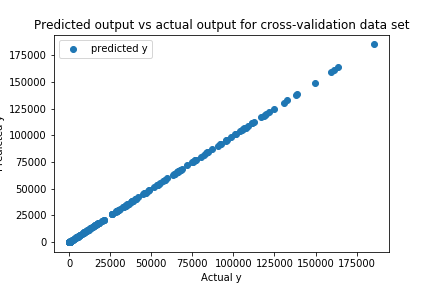
\includegraphics[scale=0.7]{images/predcv.png}
     \caption{Predicted output, Actual values for CV Data}
     \label{fig:d6500}
\end{figure}
 
\begin{figure}[H]
     \centering
     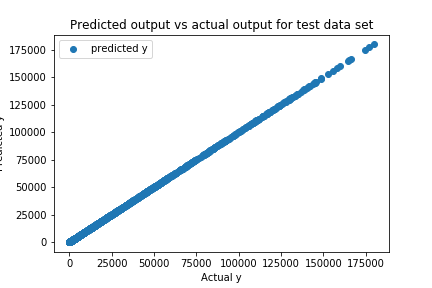
\includegraphics[scale=0.7]{images/predtest.png}
     \caption{Predicted output, Actual values for Test Data}
     \label{fig:d6500}
\end{figure}

\noi
\textbf{The surface plots of approximated functions superimposed with the scatter points are generated when the attached python code is run}
 
\section{Task 3}
Linear regression using Gaussian basis function is given as 
\begin{equation}
    y(\vec{x},\vec{w}) = \sum_{i=0}^{D-1} \omega_{i}\phi_{i}(\vec{x})
\end{equation},
where D is a hyperparameter. The basis function 
\begin{equation}
    \phi_{i} = \exp\Big(\frac{-|\vec{x} - \vec{\mu}_i|^2}{\sigma^2}\Big)
\end{equation}
where $i = 1,2 ... D-1$. The $\mu$ are the mean vectors for $D-1$ kernels made from the data set. The value of the mean vectors are found using the KMeans clustering algorithm. In this work, the \tt{sklearn} KMeans function was used. The optimum number of clusters for the dataset 2 - "\texttt{function\_12d.csv}" was found to be 10 clusters. For the dataset 3 - "\tt{1\_bias\_clean.csv}", the optimum number of clusters are 9.

\subsection{No regularization}
The following plots were obtained:
\begin{figure}[H]
     \centering
     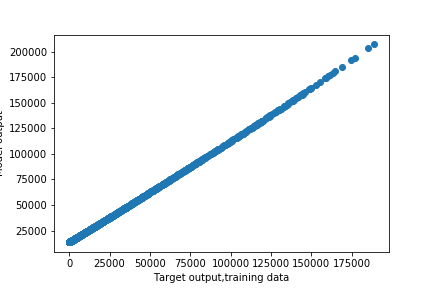
\includegraphics[scale=0.5]{images/scatter_ds2noreg.png}
     \caption{Scatter plot of the target values vs model prediction for Training set of Dataset 2, using linear regression with gaussian basis and no Regularization, $\lambda = 0.01 $}
     \label{fig:ds2tr}
\end{figure}
\begin{figure}[H]
    \centering
    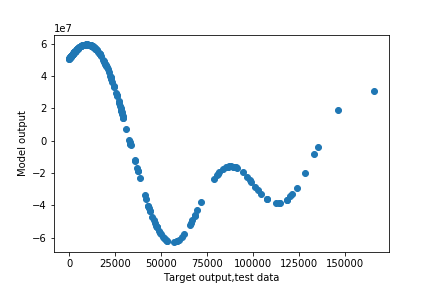
\includegraphics[scale=0.5]{images/scatter_ds2noreg_test.png}
    \caption{Scatter plot of the target values vs model prediction for Test set of Dataset 2, using linear regression with gaussian basis and no Regularization, $\lambda = 0.01 $}
    \label{fig:tikhds2tr}
\end{figure}


\subsection{Quadratic Regularization}
Optimal parameters using quadratic regularization is given by $\vec{\omega^*}$ = $(\Phi^T\Phi + \lambda I)^{-1} \Phi^T \vec{t}$;\\

\noi
$\lambda$ is the regularization parameter. The values $0.01, 0.1,  1.0, 5.0, 10.0$ were used to estimate the optimal parameters and the RMSE on the cross-validation set was calculated for each value. The best performing model was selected as the one having least RMSE on CV data \\

\noi
For dataset 2, the RMSE values for the Training, CV and Test data across $\lambda$ values is:
\def\arraystretch{1.25}
\begin{table}[H]
\centering
\begin{tabular}{l l l l}
\hline
\hline
\textbf{Lambda} & \textbf{RMSE Train} & \textbf{RMSE CV} & \textbf{RMSE Test} \\
\hline
\hline
0.01 & 3059.2231939706166 & 304419.6502059433 & 1309688.1097631603 \\
0.1 & 2967.5181829927037 & 1260.488802049498 & 41195.93571016699 \\
1.0 & 2990.3948869258456 & 1425.9232970077237 & 39596.78510421749 \\
5.0 & 3013.546633117982 & 1503.9615829712025 & 39006.81341800579 \\
10.0 & 3036.360553338793 & 1541.3504903884834 & 38684.11470986189 \\
\hline
\end{tabular}
\captionof{table}{Results obtained for Task 3}
\end{table}


\noi
Scatter plots of the model prediction using the regularization parameter value 0.01:
\begin{figure}[H]
     \centering
     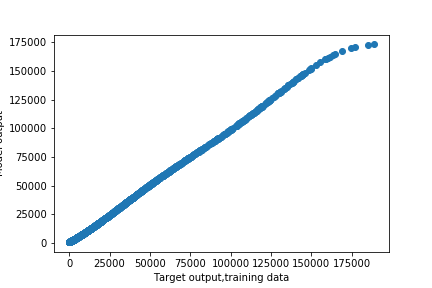
\includegraphics[scale=0.5]{images/scatter_ds2quad.png}
     \caption{Scatter plot of the target values vs model prediction for Training set of Dataset 2, using linear regression with gaussian basis and quadratic Regularization, $\lambda = 0.01 $}
     \label{fig:tikhds2tr}
\end{figure}
\begin{figure}[H]
     \centering
     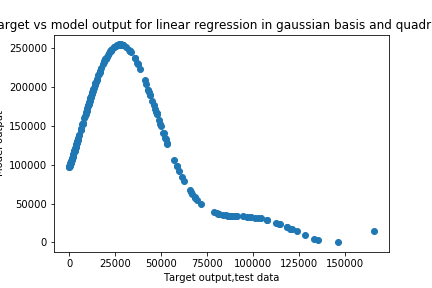
\includegraphics[scale=0.5]{images/scatter_ds2quadtest.png}
     \caption{Scatter plot of the target values vs model prediction for Test set of Dataset 2, using linear regression with gaussian basis and quadratic Regularization, $\lambda = 0.01 $}
     \label{fig:tikhds2tr}
\end{figure}
For dataset 3, the following RMSE table was obtained:
\def\arraystretch{1.25}
\begin{center}
\begin{longtable}{l l l l}
\hline
\hline
\textbf{Lambda} & \textbf{RMSE Train} & \textbf{RMSE CV} & \textbf{RMSE Test} \\
\hline
\hline
0.01 & 4929.01653053444 & 414848.3042013735 & 3312196.0992440097 \\
0.1 & 4624.091536077471 & 1669.205290237633 & 36902.34473960538 \\
1.0 & 4637.926167783597 & 2073.9375316355663 & 39568.04405922714 \\
5.0 & 4652.374704231647 & 2257.2672544567195 & 40450.17809627787 \\
10.0 & 4667.40003673528 & 2346.920490034092 & 40853.959722564214 \\
\hline
\caption{Results obtained for Task 3}
\end{longtable}
\end{center}

The scatter plots of target vs model output for the optimum value of $\lambda$ is, for "NTmin" output variable
\begin{figure}[H]
     \centering
     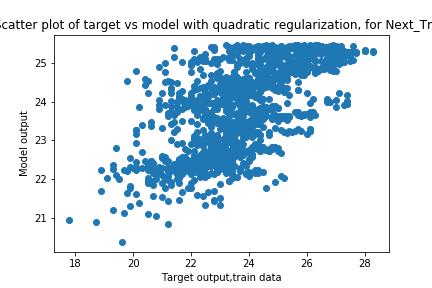
\includegraphics[scale=0.5]{images/scatter_ds3quadtrainT_min.png}
     \caption{Scatter plot of the target values vs model prediction for Training set of Dataset 3, using linear regression with gaussian basis and quaadratic Regularization, $\lambda = 0.01 $ for "NTmin" output variable}
     \label{fig:tikhds2tr}
\end{figure}
\begin{figure}[H]
     \centering
     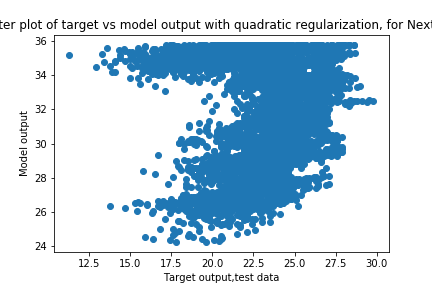
\includegraphics[scale=0.5]{images/scatter_ds3quadtestT_min.png}
     \caption{Scatter plot of the target values vs model prediction for Test set of Dataset 2, using linear regression with gaussian basis and quadratic Regularization, $\lambda = 0.01 $, for "NTmin" output variable}
     \label{fig:tikhds2tr}
\end{figure}
For "NTmax":
\begin{figure}[H]
     \centering
     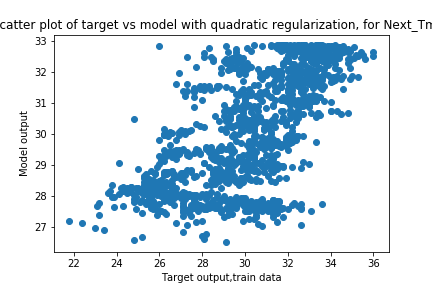
\includegraphics[scale=0.5]{images/scatter_ds3quadtrainT_max.png}
     \caption{Scatter plot of the target values vs model prediction for Training set of Dataset 3, using linear regression with gaussian basis and quaadratic Regularization, $\lambda = 0.01 $ for "NTmax" output variable}
     \label{fig:tikhds2tr}
\end{figure}
\begin{figure}[H]
     \centering
     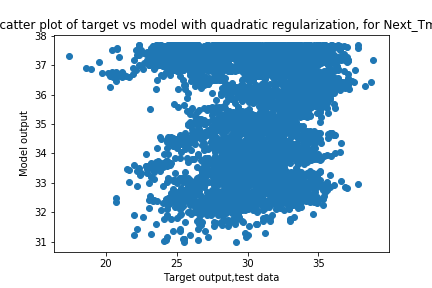
\includegraphics[scale=0.5]{images/scatter_ds3quadtestT_max.png}
     \caption{Scatter plot of the target values vs model prediction for Test set of Dataset 2, using linear regression with gaussian basis and quadratic Regularization, $\lambda = 0.01$, for "NTmax" output variable}
     \label{fig:tikhds2tr}
\end{figure}

\subsection{Tikhonov Regularization} 
The Tikhonov regularization term is given by $\vec{\omega^*}$ = $(\Phi*T\Phi + \lambda \Tilde{\Phi})^{-1} \Phi^T \vec{t}$. The $\Tilde{\Phi}$ term is defined as 
\begin{equation}
    \Tilde{\Phi} = [\Tilde{\phi}]_{i,j = 1}^{K}
\end{equation}

where K is the number of clusters and $\lambda$ is the regularization parameter. The values 0.01,0.1, 1.0,5.0,10.0 were used to estimate the optimal parameters and the RMSE on the cross-validation set was calculated for each value. The best perorming model was selected as the one having least RMSE on CV data\\ 
Applying Tikhonov regularization to the bivariate dataset, the optimal value of $\lambda$ was estimated to be 0.01. 
 The table for the RMSE values for the Training, CV and Test values corresponding to each $\lambda$ value is
\def\arraystretch{1.25}
\begin{table}[H]
\centering
\begin{tabular}{l l l l}
\hline
\hline
\textbf{Lambda} & \textbf{RMSE Train} & \textbf{RMSE CV} & \textbf{RMSE test} \\
\hline
\hline
0.01 & 78112040.25241715 & 80416219813.42682 & 43898825037.538 \\
0.1 & 78629878.58895023 & 276304216179.1798 & 176596027875.55765 \\
1.0 & 79471104.52781227 & 357583741029.9827 & 104372422450.83612 \\
5.0 & 77593937.82583737 & 272444591755.6569 & 174802698267.85687 \\
10.0 & 77693846.61754198 & 242869557997.72043 & 158196054705.92648 \\
\hline
\end{tabular}
\caption{Results obtained for Task 3}
\end{table}


\noi
Scatter plots of the model prediction using the regularization parameter value 0.01:
\begin{figure}[H]
     \centering
     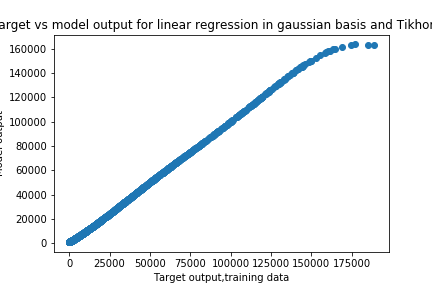
\includegraphics[scale=0.5]{images/scatter_ds2tikhtr.png}
     \caption{Scatter plot of the target values vs model prediction for Training set of Dataset 2, using linear regression with gaussian basis and Tikhonov Regularization, $\lambda = 0.01 $}
     \label{fig:tikhds2tr}
\end{figure}
\begin{figure}[H]
     \centering
     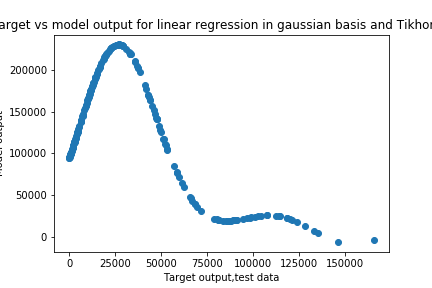
\includegraphics[scale=0.5]{images/scatter_ds2tikhtest.png}
     \caption{Scatter plot of the target values vs model prediction for Test set of Dataset 2, using linear regression with gaussian basis and Tikhonov Regularization, $\lambda = 0.01 $}
     \label{fig:tikhds2tr}
\end{figure}

 \noi
For Dataset 3, the table for the RMSE values for the Training, CV and Test values corresponding to each $\lambda$ value corresonding to target variable "NTmin" is\\
\def\arraystretch{1.25}
\begin{center}
\begin{longtable}{l l l l}
\hline
\hline
\textbf{Lambda} & \textbf{RMSE Train} & \textbf{RMSE CV} & \textbf{RMSE test} \\
\hline
\hline
0.01 & 4929.01653053444 & 414848.3042013735 & 3312196.0992440097 \\
0.1 & 4624.091536077471 & 1669.205290237633 & 36902.34473960538 \\
1.0 & 4637.926167783597 & 2073.9375316355663 & 39568.04405922714 \\
5.0 & 4652.374704231647 & 2257.2672544567195 & 40450.17809627787 \\
10.0 & 4667.40003673528 & 2346.920490034092 & 40853.959722564214 \\
\hline
\end{longtable}
\setcounter{table}{0}
\captionof{table}{Results obtained for Task 3}
\end{center}


\noi
the optimal value of $\lambda$ was estimated to be 0.1 for the target output "NTmin". The scatter plots obtained are Figures \ref{fig:tikhds3tr} and \ref{fig:tikhds3t}
\begin{figure}[H]
     \centering
     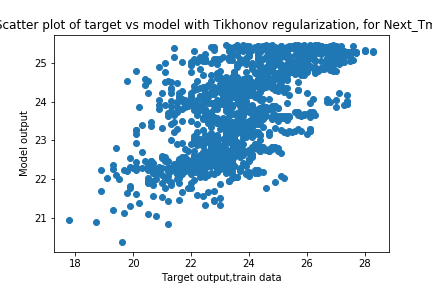
\includegraphics[scale=0.5]{images/scatter_ds3tikhtrainT_min.png}
     \caption{Scatter plot of the target values vs model prediction for Training set of Dataset 3, using linear regression with gaussian basis and Tikhonov Regularization, $\lambda = 0.1 $}
     \label{fig:tikhds3tr}
\end{figure}
\begin{figure}[H]
     \centering
     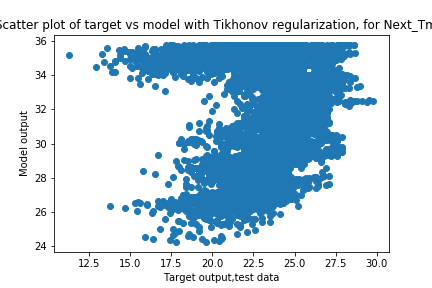
\includegraphics[scale=0.5]{images/scatter_ds3tikhtestT_min.png}
     \caption{Scatter plot of the target values vs model prediction for Test set of Dataset 3, using linear regression with gaussian basis and Tikhonov Regularization, $\lambda = 0.01 $}
     \label{fig:tikhds3t}
\end{figure}
 For the target output "NTmax" the following table of RMSE values for the training, test and CV data was obtained:
\def\arraystretch{1.25}
\begin{table}[H]
\centering
\begin{tabular}{l l l l}
\hline
\hline
\textbf{Lambda} & \textbf{RMSE Train} & \textbf{RMSE CV} & \textbf{RMSE test} \\
\hline
\hline
0.01 & 4929.01653053444 & 414848.3042013735 & 3312196.0992440097 \\
0.1 & 4624.091536077471 & 1669.205290237633 & 36902.34473960538 \\
1.0 & 4637.926167783597 & 2073.9375316355663 & 39568.04405922714 \\
5.0 & 4652.374704231647 & 2257.2672544567195 & 40450.17809627787 \\
10.0 & 4667.40003673528 & 2346.920490034092 & 40853.959722564214 \\
\hline
\end{tabular}
\caption{Results obtained for Task 3}
\end{table}

 plots were obtained: figures \ref{fig:tikhds3tr2} and \ref{fig:tikhds3t2}.
\begin{figure}[H]
     \centering
     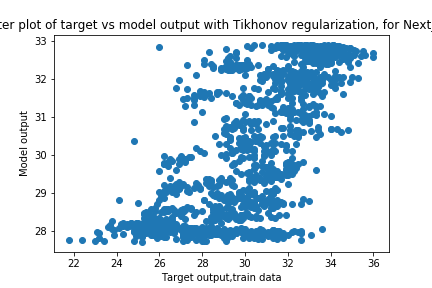
\includegraphics[scale=0.5]{images/scatter_ds3tikhtrainT_max.png}
     \caption{Scatter plot of the target values vs model prediction for Training set of Dataset 3, using linear regression with gaussian basis and Tikhonov Regularization, $\lambda = 0.1 $}
     \label{fig:tikhds3tr2}
\end{figure}
\begin{figure}[H]
     \centering
     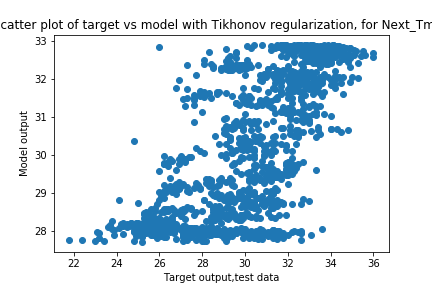
\includegraphics[scale=0.5]{images/scatter_ds3tikhtestT_max.png}
     \caption{Scatter plot of the target values vs model prediction for Test set of Dataset 3, using linear regression with gaussian basis and Tikhonov Regularization, $\lambda = 0.1 $}
     \label{fig:tikhds3t2}
\end{figure}

% \break
% \bibliographystyle{unsrt}
% \bibliography{reference}
\end{document}